\documentclass[a4paper, 11pt]{article}
\usepackage{comment} % enables the use of multi-line comments (\ifx \fi) 
\usepackage{fullpage} % changes the margin
\usepackage[german]{babel}
\usepackage[utf8]{inputenc}
\usepackage{graphicx}
\usepackage{multicol}
\usepackage{float}
\usepackage{fancyhdr}
\usepackage{enumitem}
\pagestyle{fancy} 
\usepackage{pdfpages}
%\usepackage[head=128pt]{geometry}
\title{Sitzungs-protokoll}
\author{Christian Kirfel}
\usepackage[margin=1in]{geometry}
\setlength{\footskip}{0.1pt}
\setlength{\headheight}{80pt}
\setlength{\topmargin}{0pt}
\setlength\parindent{0pt}
\fancypagestyle{style1}{
\rhead{
\includegraphics[width=4cm]{logo_catena}}
\cfoot{
\makebox{}\\
\makebox{}\\
\hspace{15cm}
\makebox[0.1\linewidth]{\rule{0.1\linewidth}{0.1pt}} \hspace{1cm} \makebox[0.1\linewidth]{\rule{0.1\linewidth}{0.1pt}} \hspace{1cm} \makebox[0.1\linewidth]{\rule{0.1\linewidth}{0.1pt}} \hspace{1cm} \makebox[0.1\linewidth]{\rule{0.1\linewidth}{0.1pt}} \hspace{1cm}\\}
}

\newcommand\signature[2]{% Name; Department
\noindent\begin{minipage}{5cm}
    \noindent\vspace{3cm}\par
    \noindent\rule{5cm}{1pt}\par
    \noindent\textbf{#1}\par
    \noindent#2%
\end{minipage}}



\begin{document}
\pagestyle{style1}

\textbf{Datum: 06.11.2021} % inserir data aqui
\textbf{Sitzungszeit: 13:00 - 13:50}
\textbf{Ort: Remote, Zoom} % Definir local da reunião 

\textbf{Teilnehmer:} %
\begin{description}
\item Yannick Hansen, Vorsitzender
\item Dr.~Michael Schumacher, stellv. Vorsitzender
\item Volker Nießen, Geschäftsführer
\item Friedhelm Schmitt, Schatzmeister
\item Christian Kirfel, Schriftführer
\item Jörg Zwitters, Verbindungslehrer/Beisitzer
\item Leonhard Paulig, Kassenprüfer
\item Sebastian Heinen, Kassenprüfer
\item Dominik Hoven, Beisitzer
\item Martin Reinicke, Beisitzer
\item Max Frauenrath, Beisitzer
\item Philip Lanio, Beisitzer
\item Kimberly Sarlette, SV-Verbindung
\item Thomas Frauenkron
\item Dirk Udo Fricke
\item Günter M. Lutsch
\item Alfred Kahl
\item Anja Pick
\item Burkhard Cremer
\item J. Boshold
\item Lothar Esser
\item Martin Heinen
\item Hermann Preußner
\item Rudolf Gerhards
\item Stefan Mathey
\item Thomas Webr
\item Wolfgang Bergsdorf
\item Wolfgang Schmitz
\item Clara Keutgen
\item Ute Stolz
\end{description}

\makebox[\linewidth]{\rule{\linewidth}{0.4pt}}\\
\textbf{Programmpunkte:} 
\begin{enumerate}
\item Begrüßung
\item Feststellung der Beschlussfähigkeit
\item Genehmigung des Protokolls der MV September 2020
\item Bericht des Vorstandes
\item Bericht des Vorsitzenden
\item Bericht des Schatzmeisters
\item Bericht des Kassenprüfers
\item Entlastung des Vorstandes
\item Wahl des Vorstandes
\item Verschiedenes
\item Persönliche Anträge
\end{enumerate}
\makebox[\linewidth]{\rule{\linewidth}{0.4pt}}\\

\newpage

\section*{Begrüßung}

Die Hauptversammlung findet wegen Covid 19 hybrid statt. Der analoge Teil sitzt in Steinfeld.
Yannick Hansen erinnert an die im Anschluss stattfindende Veranstaltung zur Feier des 40-jährigen Vereinsjubiläums.


\section*{Beschlussfähigkeit}

Für Kommentare muss über Zoom reagiert werden.

Die Beschlussfähigkeit wird auf Antrag des Vorsitzenden festgestellt.

\section*{Genehmigung des Protokolls der MV September 2020}

Das Protokoll wird ohne Widerspruch genehmigt.

\section*{Bericht Schule}

Jörg Zwitters berichtet über das Schulleben im vergangenen Jahr.
Corona hat auch Steinfeld und das Schulleben im Griff.
Durch den Lockdown fand viel Unterricht digital statt.
Durch die Digitalisierung der Schule war der Unterrich von zuhause sehr erfolgreich und es wurde vom Digitalpakt profitiert.
Durch den Digitalpakt ist noch mehr Geld in die Schule geflossen. Zwischen den access points wurde unter Pater Pauls Leitung Glasfaser gelegt.
Der erste Ipad Jahrgang hat Abiur gemacht.
Die Sportstätten auf dem Außengelände wurden ausgebaut, inklusive Laufbahn, Kugelstoßen und Weitsprung.
Die Segel AG konnte nicht regelmäßig stattfinden und die Amadeus steht seit zwei Jahren in der Scheune.
Bald kann das Projekt hoffentlich wieder anlaufen.

\section*{Bericht Stiftung}

Martin Reinicke berichtet.
Die Stiftung ist im Prozess sich digital weiterzuentwickeln. Website und Kapitalerhalt sollten erneuert werden.
Die Stifutng sollte bald in der Lage sein die Schule langfristig zu unterstützen.

\section*{Schülervertretung}

Kimberly Sarlette übernahm die Kommunikation mit der SV im letzten Jahr.
Eine neue SV wurde gewählt. 10 Schüler besuchten ein Seminar über Ideen und Grundlagen für eine Schülervertretung.
Die ehemalige SV hat einen Zukunftstag organisiert.

\section*{Berufsberatung}

Dominik Hoven ist der Ansprechpartner für Berufsberatung.
Nach den Weihnachtsferien sind einführende Vorträge zu Studium, work and travel und Ausbildung geplant.
Ein besonderer Fokus liegt auf den alltäglichen Dingen von Geldkosten bis Sportveranstaltungen.
Yannick, Kimberly, Martin und Max haben besprochen was die wichtigen Infos sind, die uns selber gefehlt haben.
Yannick fügt hinzu, dass die Resonanz seitens der Schule sehr positiv war.

\section*{Kurse und Vorträge}

Christian Kirfel berichtet über geplante Vorträge und Kurse für Schüler und Ehemalige aus allen Fachbereichen der Catena Mitglieder.
So soll auch der Fokus auf Ehemalige neben der Schulförderung verstärkt werden. 
Corona ist hier ein hemmender Faktor.

\section*{Segel AG}

Ein genauer Bericht über die Segel AG wird auf die anschließende Veranstaltung verlegt.

\section*{Bericht des Vorsitzenden}


Yannick Hansen berichtet, dass er die aktuelle Website selbst betreibt.
Ein modernes Design und Automatisierung, unter anderem eines Newsletters, sind so gewährleistet.
Die Blogeinträge werden ebenfalls aktueller gehalten.
Ein weiteres Ziel ist die effizientere Kommunikation und Anmeldung zu geplanten Veranstaltungen.

Auch zur Mitgliederverwaltung besteht neue software. Durch eine Dezentralisierung kann die Arbeit auf mehrere Vorstandsmitglieder aufgeteilt werden.
Volker Nießen kann so die Arbeit der Mitgliederverwaltung wieder aufnehmen.
Die Stammdaten im Verein können nun digital von den Mitgliedern selber kontrolliert werden.

Das neue Newsletter Programm ist Rapidmail. Es handelt sich wie bei der Website um ein Baukastensystem, dass das einfache Versenden schöner Newsletter erlaub
Diese werden direkt in das Mitgliedersystem eingespeist

Außerdem hat die Catena die Schule beim Bau einer Calisthenics Anlage unterstützt.
Diese wurden unter anderem von den Sportlehrern aufgebaut.

Außerdem trägt der Vorstand bereits Polos die bald für alle geplant sind.

In den kommenden Jahren möchte die Catena präsenter für die Schüler sein. Vor allem in Hibnlick auf Berusberatung.
Nächstes Jahr hoffen wir wieder in Person in Steinfeld mit dem Mitgliedern feiern zu können.
Ein Sv Ausflug ist auch erneut geplant.




\section*{Bericht des Schatzmeisters}

Kassenbericht des letzten Jahres, wird in der Präentation gezeigt und hier übernommen. (Abbidlugen \ref{fig:kasse1}, \ref{fig:kasse2} und \ref{fig:kasse3})

\begin{figure}
    \centering
    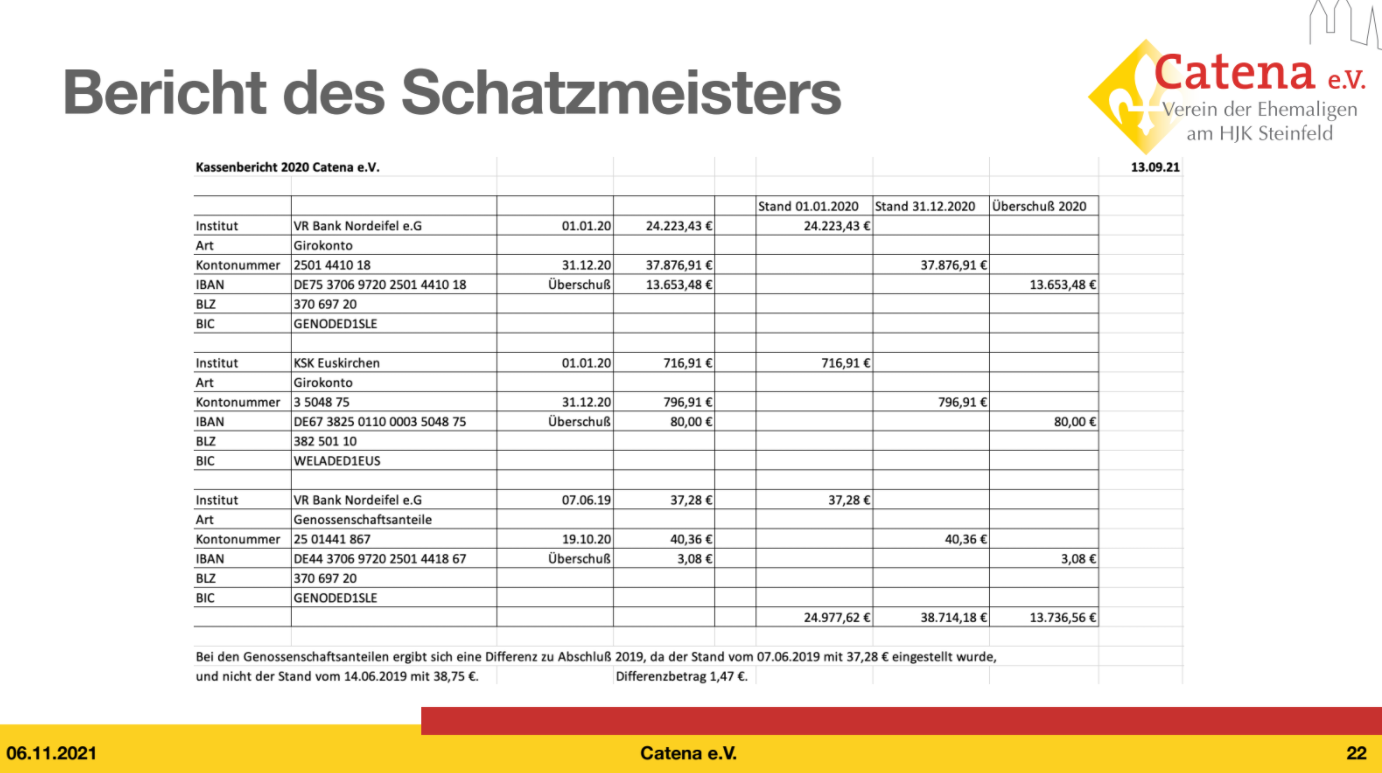
\includegraphics[width=0.8\textwidth]{schatz1}
    \caption{Bericht des Schatzmeisters, entnommen aus den Folien aus der Hauptversammlung.}
    \label{fig:kasse1}
\end{figure}

\begin{figure}
    \centering
    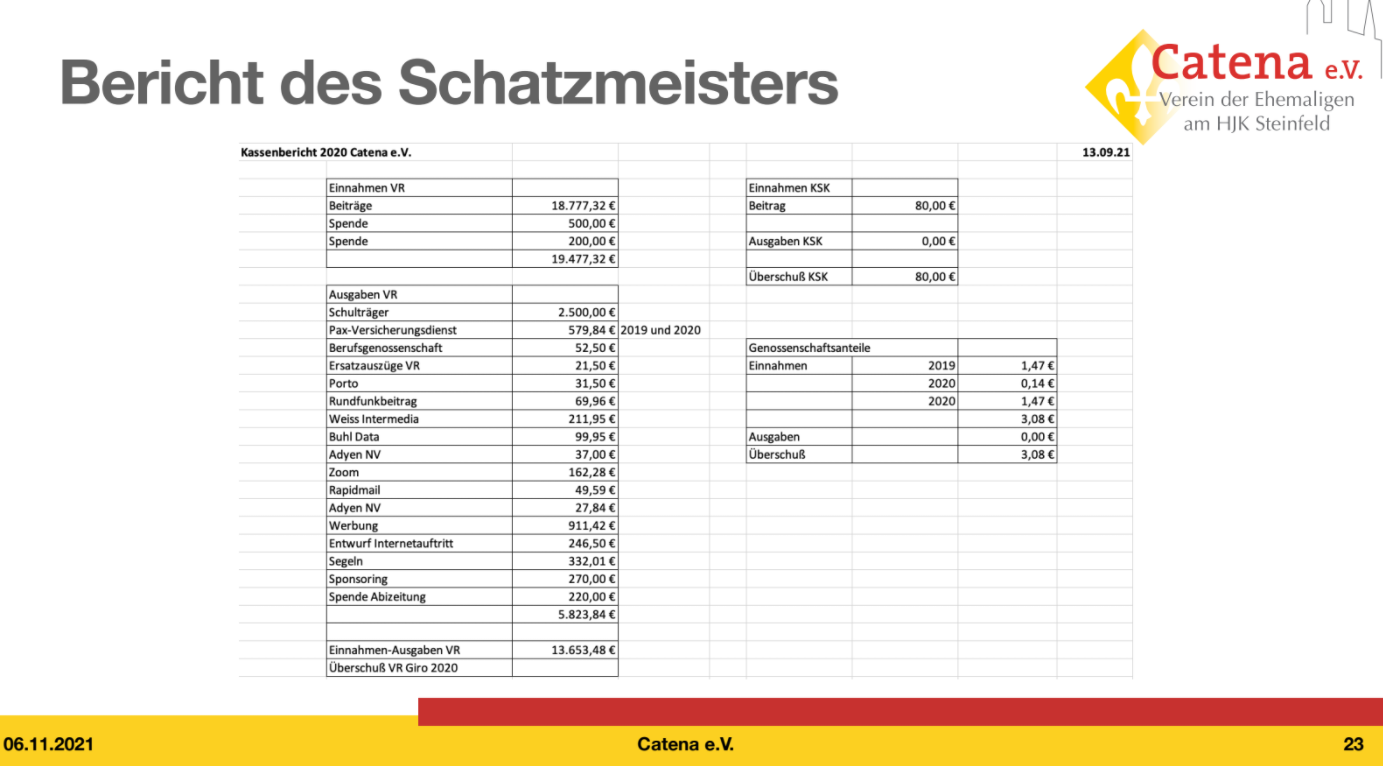
\includegraphics[width=0.8\textwidth]{schatz2}
    \caption{Bericht des Schatzmeisters, entnommen aus den Folien aus der Hauptversammlung.}
    \label{fig:kasse2}
\end{figure}

\begin{figure}
    \centering
    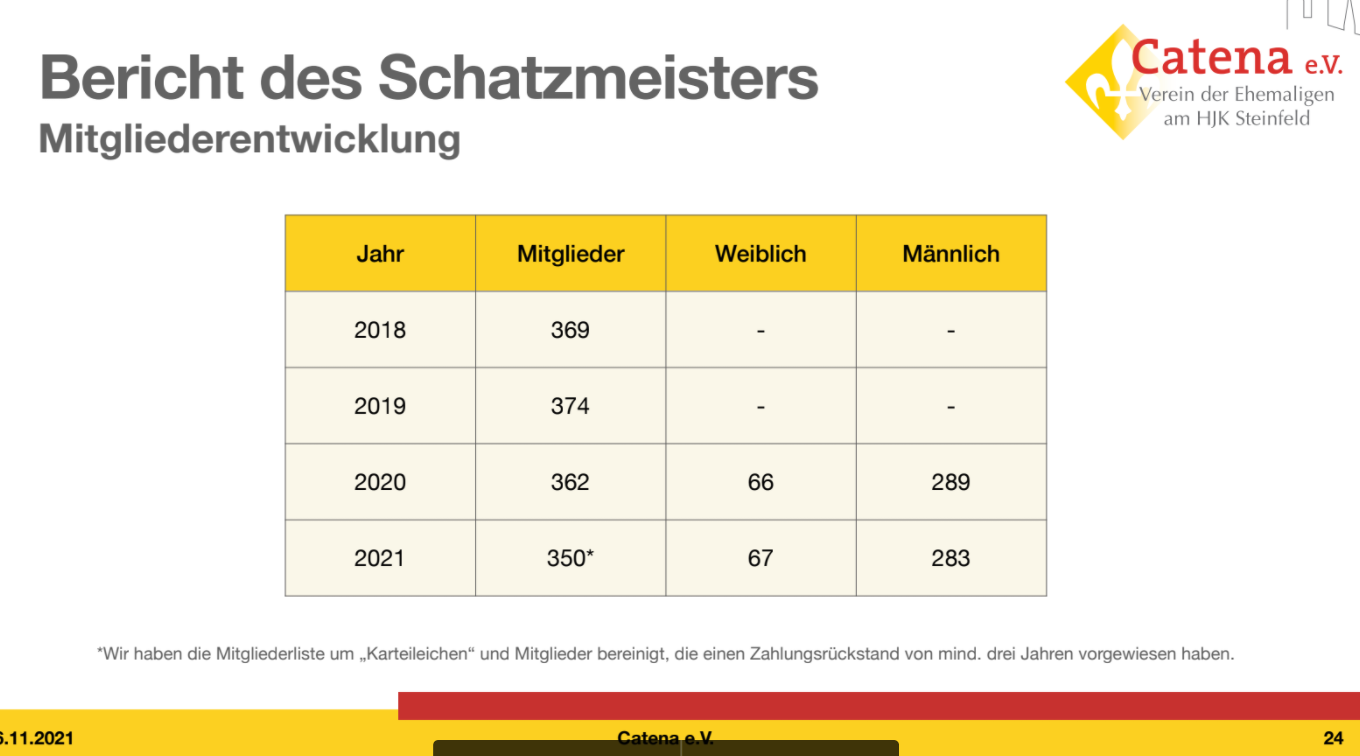
\includegraphics[width=0.8\textwidth]{schatz3}
    \caption{Bericht des Schatzmeisters, entnommen aus den Folien aus der Hauptversammlung.}
    \label{fig:kasse3}
\end{figure}


\section*{Bericht des Kassenprüfers}

Leonhard Paulig hat den Bericht verschickt.
Als zweiter Prüfer wurde Sebastian Heinen im Vorhinein per Vorstandsbeschluss bestimmt.
Er hat mit Sebastian Heinen die Zahlen geprüft.
Corona-bedingt wurde viel gespart aber die Finanzen wurden ordentlich geführt.



\section*{Entlastung des Vorstandes}

Es gibt keine Gegenstimmen zur Entlastung des Vorstandes. Damit wird der Vorstand mit Bestätigung des Protokolls entlastet.

\section*{Wahl des Vorstands}

\subsection*{Wahl der Vorsitzenden}

Leonahrd Paulig leitet die Wahl der Vorsitzenden.
Keine Gegenstimmen für Yannick Hansen.
Yannick Hansen nimmt die Wahl an.

\subsection*{Wahl des Vorstands}

Der stellvertretdende Vostizende Dr.~Michael Schumacher tritt zurück.
Kimberly Sarlette wird vorgeschlagen.
Es gibt keine Gegenvorschläge
es gibt keine Gegenstimmen.
Es gibt keine Enthaltungen.
Kimberly Sarlette nimmt die Wahl an.
Volker Nießen wird als Geschäftsführer vorgeschlagen.
Es gibt keine Gegenvorschläge.
Es gibt keine Gegenstimmen.
Voker nimmt die Wahl an.
Friedhelm Schmitt tritt als Schatzmeister zurück.
Sebastian Heinen wird als neuer Kandidat vorgeschlagen.
Sebastian Heinen stellt sich kurz vor.
Es gibt keine Gegenvorschläge.
Es gibt keine Gegenstimmen.
Sebastian nimmt die wahl an.
Der Schriftführer, Christian Kirfel, und alle Beistzer werden erneut vorgeschlagen.
Es gibt keine Gegenvorschläge.
Es gibt keine Gegenstimmen.
Alle nehmen die Wahl an.
Nicht Anwesende haben die Wahl bereits schriftlich angenommen.


\section*{Wahl des Kassenprüfers}
Leonhard Paulig steht zur Verfügung.
Als zweiter Prüfer wird Michael Schumacher vorgeschagen.
Leonhard nimmt die wahl ohne Gegenstimmen an.
Michael steht zur Verfügung.
Es gibt keine anderen Vorschläge oder Gegenstimmen.
Michael nimmt die wahl an.

\section*{Verschiedenes}

\section*{Persönliche Anträge}

\newpage

Protokoll: Christian Kirfel


\signature{Yannick Hansen}{Vorsitzender}\hfill\signature{Christian Kirfel}{Schriftführer}


\end{document}